\documentclass[api,pof,pre,12pt,a4paper]{revtex4-1}     
\usepackage{bm}
\usepackage{natbib}
\usepackage{url}
\usepackage[intlimits]{amsmath}
\usepackage{graphicx}
\usepackage{fancyhdr}
\usepackage{amsfonts}
\usepackage{amssymb}
%\usepackage{pstricks}
%\usepackage{pst-coil}
%\usepackage{pst-plot}
\usepackage{hyperref}
\usepackage{float}
\usepackage{subfig}


\newtheorem{theorem}{Theorem}
\newtheorem{prob}{Problem}
\newenvironment{problem}[1]{\begin{prob} {\rm #1} \end{prob}}

%Nadir's Shortcuts
\newcommand{\beqn}{\begin{equation}}
\newcommand{\eeqn}{\end{equation}}
\newcommand{\beqa}{\begin{eqnarray}}
\newcommand{\eeqa}{\end{eqnarray}}
\newcommand{\beqanonum}{\begin{eqnarray*}}
\newcommand{\eeqanonum}{\end{eqnarray*}}
\newcommand{\beqnonum}{\begin{equation*}}
\newcommand{\eeqnonum}{\end{equation*}}
\newcommand{\jump}{\vspace{0.5cm}}
\newcommand{\bbf}{\begin{bf}}
\newcommand{\ebf}{\end{bf}}
%\newcommand{\eqnref}[1]{(\ref{#1})}
\newcommand{\defn}[1]{\begin{bf}\emph{#1}\end{bf}}
\newcommand{\reals}{\ensuremath{\mathbb{R}}}
\newcommand{\complex}{\ensuremath{\mathbb{C}}}
\newcommand{\integers}{\ensuremath{\mathbb{Z}}}
\newcommand{\half}{\ensuremath{\frac{1}{2}}}
\newcommand{\n}{\nonumber}
\renewcommand{\d}{\mathrm{d}}
\newcommand{\del}{\partial}
\newcommand{\dd}{\ensuremath{\, \mathrm{d}}}
\newcommand{\nint}[4]{\int_{#3}^{#4} {#1}\, \mathrm{d}{#2}}
\newcommand{\der}[2]{\frac{\d {#1}}{\d {#2}}}
\newcommand{\parder}[2]{\frac{\del {#1}}{\del {#2}}}
\newcommand{\funder}[2]{\frac{\delta {#1}}{\delta {#2}}}
\newcommand{\Lag}{\mathcal{L}}


% Draft macros
\newcommand{\TODO}[1]{\marginpar{\raggedright\scriptsize\textbf{TODO:} #1} (\textbf{TODO})}
\newcommand{\NOTE}[1]{\marginpar{\footnotesize\textbf{NOTE}} (\textbf{#1})}


\oddsidemargin  0.0in
\evensidemargin 0.0in
\textwidth      6.5in
\headheight     15pt
\topmargin      0.0in
\textheight=8.0in
%\setlength{\parindent}{0in}

\lhead{Wavelength competition in modified SH}
\chead{}
\rhead{Gandhi et al.}
%\lfoot{}
%\cfoot{}
%\rfoot{}


%Figures
\newcommand{\FIGmarginalstability}{
\begin{figure}[h]\center
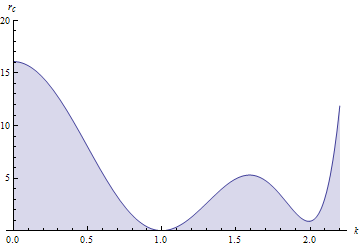
\includegraphics[width=60mm]{MarginalStability.png}
\caption{\label{fig:marginalstability} Linear stability of the modified Swift-Hohenberg equation with $q=2$ and $\delta=.1$.  The shaded region indicates linearly stable parameter regimes of the homogeneous solution with a forcing $r$ for a given wavenumber $k$.}
\end{figure}
}
\newcommand{\FIGbifurcationdiagramA}{
\begin{figure}[h]\center
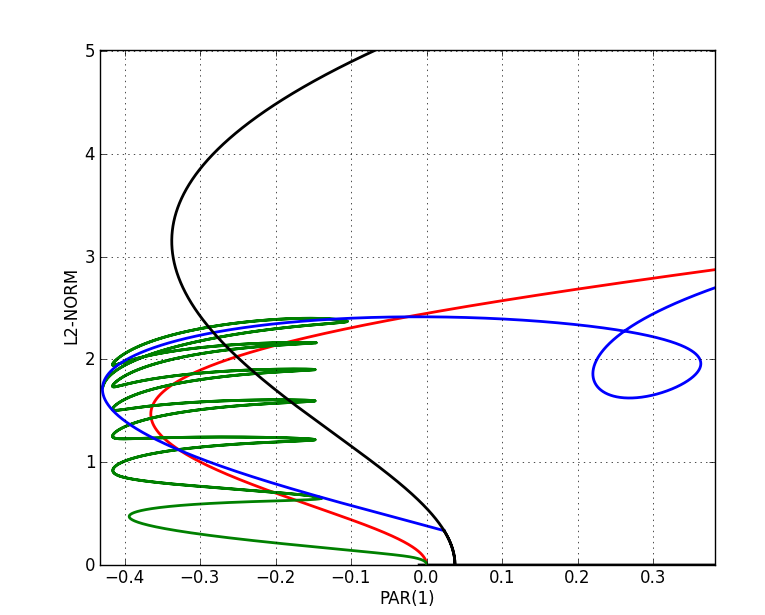
\includegraphics[width=120mm]{BifurcationDiagram1.png}
\caption{\label{fig:bifurcationdiagram1} A Bifurcation diagram for the case that $q=1$ and $\delta=0$, showing a snaking branch that connects two periodic states.}
\end{figure}
}

\newcommand{\FIGdoubleperiod}{
\begin{figure}[h]
  \begin{center}
    \mbox{
      \subfloat[solution before the loop]{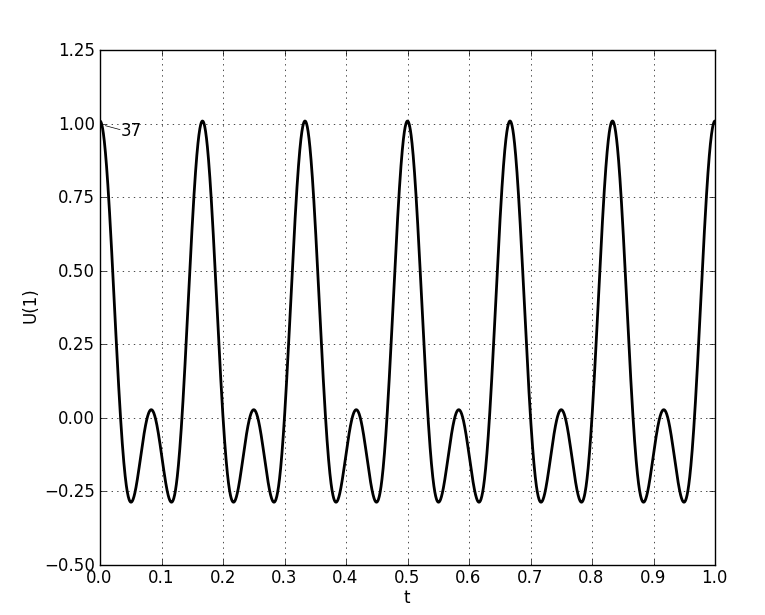
\includegraphics[width=60mm]{dpb24.png}} \quad
      \subfloat[solution after the loop]{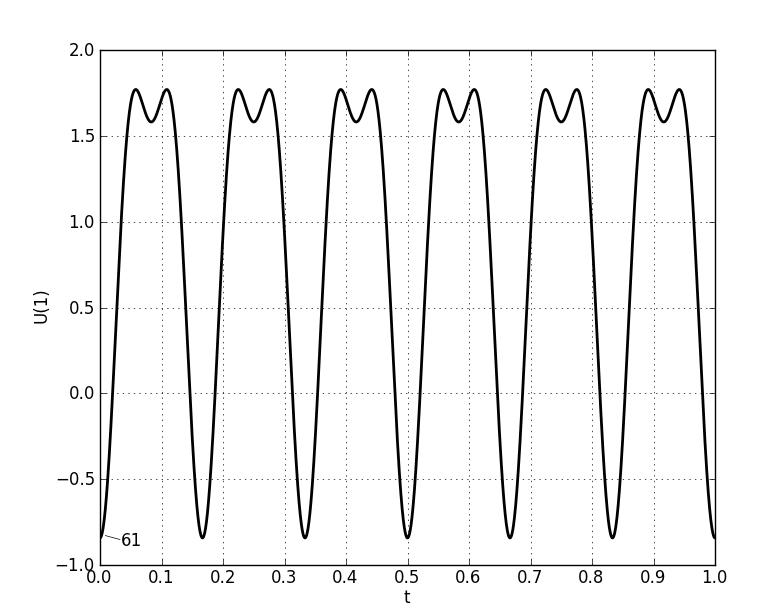
\includegraphics[width=60mm]{dpb24u.png}} 
      }
    \caption{Solutions along periodic branch that bifurcations from $P24$ and connects with the snaking branch from $P20$.}
    \label{fig:doubleperiod1}
  \end{center}
\end{figure}
}

\newcommand{\FIGsnakingA}{
\begin{figure}[h]
  \begin{center}
    
      \subfloat[1]{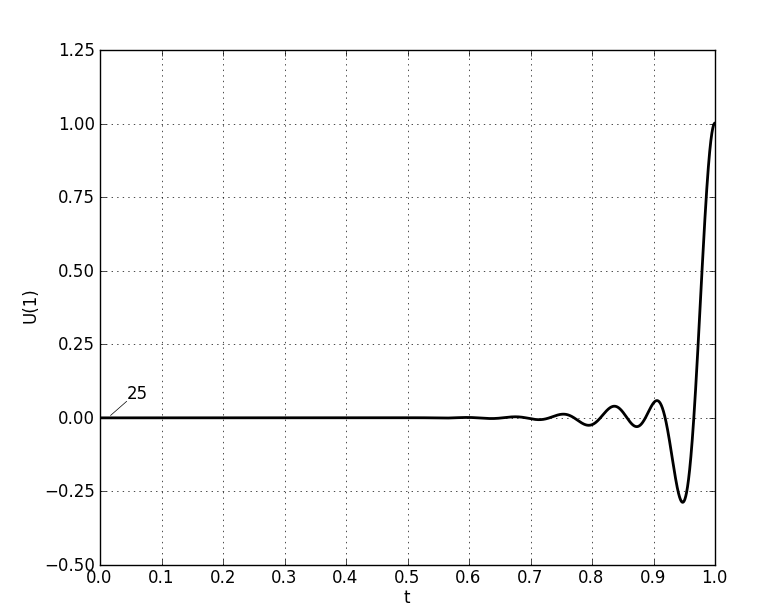
\includegraphics[width=60mm]{sb20a1.png}} \quad
      \subfloat[2]{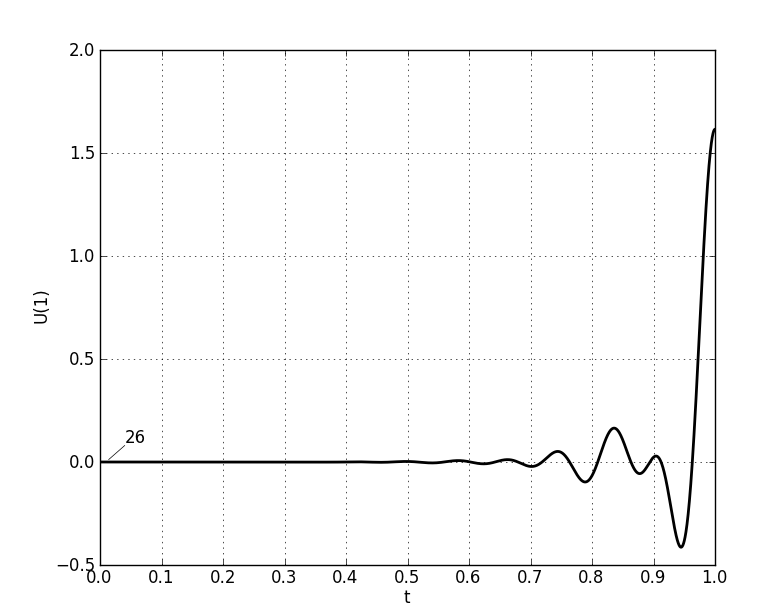
\includegraphics[width=60mm]{sb20a2.png}}\\
      \subfloat[3]{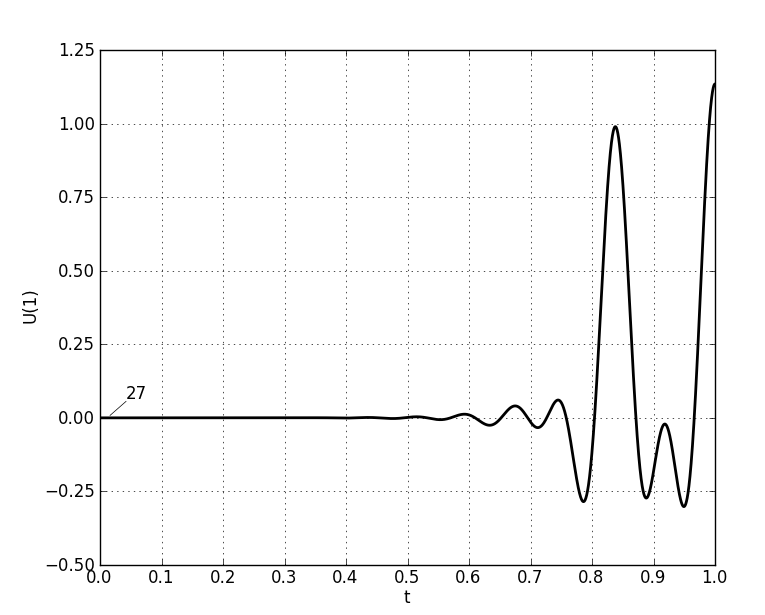
\includegraphics[width=60mm]{sb20a3.png}} \quad
      \subfloat[4]{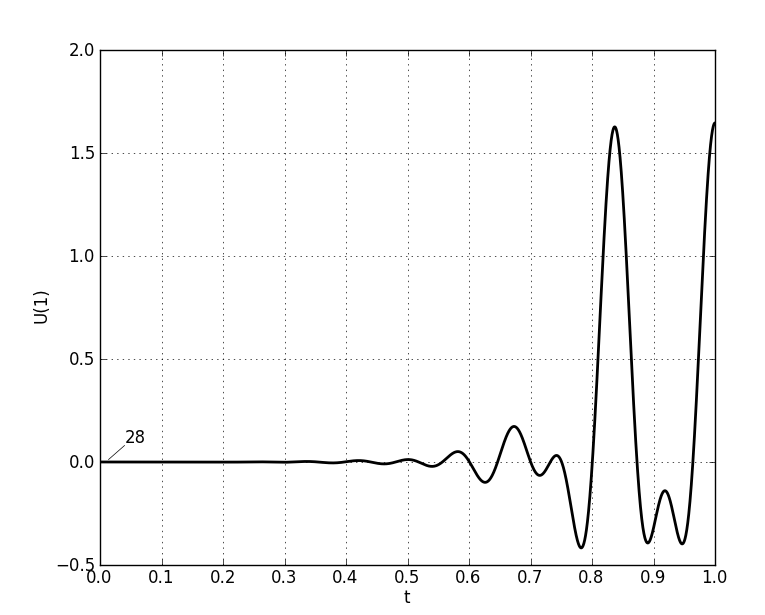
\includegraphics[width=60mm]{sb20a4.png}} 
      
    \caption{Localized solutions along snaking branch that bifurcates from $P20$.}
    \label{fig:snaking1}
  \end{center}
\end{figure}
}


\newcommand{\FIGsnakingmess}{
\begin{figure}[h]
  \begin{center}
    \mbox{
      \subfloat[Example solution from third bifurcation point along $P20$]{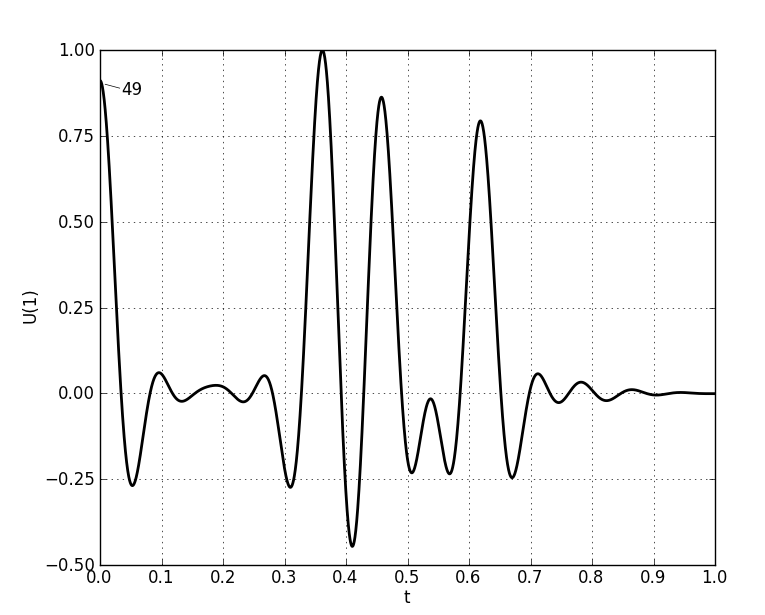
\includegraphics[width=60mm]{sb20cMess.png}} \quad
      \subfloat[Example solution from second bifurcation point along $P24$]{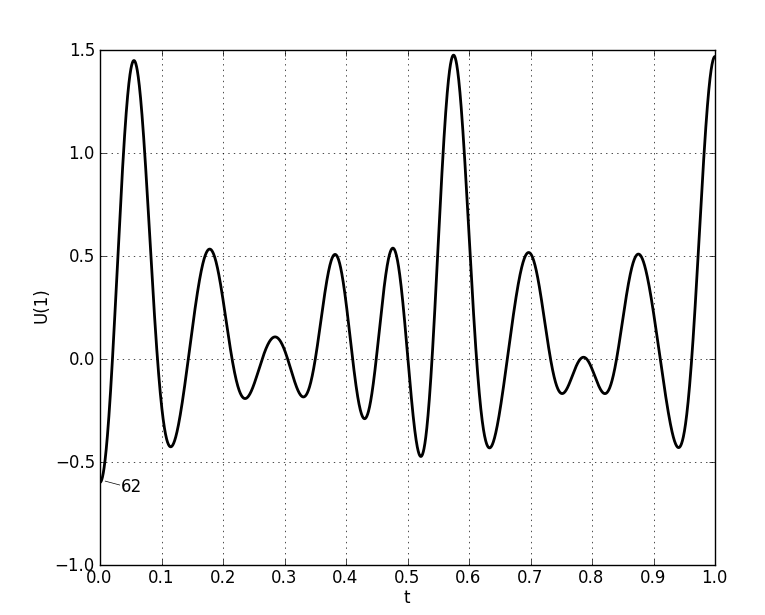
\includegraphics[width=60mm]{sb24bMess.png}} 
      }
    \caption{Examples of solutions with seemingly random pulses. These solutions fall along messy branches that bifurcate from the primary periodic solutions}
    \label{fig:snakingmess1}
  \end{center}
\end{figure}
}


\pagestyle{fancy}
\begin{document}
\preprint{APS/123-QED}

\title{Pattern Formation in a system with competing wavelengths}

\author{Punit Gandhi}
 \email{punit_gandhi@berkeley.edu}
\author{Edgar Knobloch}
 \email{knobloch@berkeley.edu}
\affiliation{Department of Physics, University of California, Berkeley CA 94720, USA}

\begin{abstract}
We propose a modified version of the Swift-Hohenberg equation in an attempt to study a situation in which competition between two patterns of different wavelength exist.
\end{abstract}

\maketitle

\section{Introduction}
The Swift-Hohenberg equation serves as a model for pattern formation in a broad range of physical systems.   This equation, which takes the form  
\begin{equation}
u_t= r u-\left(1+\partial_{x}^2\right)^2u+N[u]\label{eq:SH},
\end{equation}
describes the dynamics of a real field $u$ over one spatial dimension in time, where $N$ is some nonlinear function of $u$.  We have rescaled the equation so that the critical wavenumber that defines the natural wavelength of the patterned state is unity.  We will be interested in two possible choices of $N$, namely $N_{23}[u]=bu^2-u^3$ and $N_{35}[u]=b u^3-u^5$.  The strength of the linear forcing term $r$ and the strength of the quadratic nonlinearity $b$ are left as parameters of the system.  

There may be physical systems in which multiple patterned states with different characteristic wavelengths can exist simultaneously.  We would like to develop a model for such a system and study the interaction and competition between these patterned states.  We propose a modification to the Swift-Hohenberg equation in which such competition may be possible:
\begin{equation}
u_t= r u-\left(1+\partial_{x}^2\right)^2 \left[\left(q^2+\partial_{x}^2\right)^2+\delta \right] u+N[u]\label{eq:SHm}.
\end{equation}
Linear stability analysis of this equation results in a marginal stability curve (Fig. \ref{fig:marginalstability}) where two wavelengths can compete with each other.  The first wavelength is  $k=1$, just as in the original SHE (Eq.~\ref{eq:SH}), and the other occurs at 
\beqn
q_*=\frac{1}{2}\sqrt{1+3q^2 \pm\Delta}.
\eeqn
where $\Delta=\sqrt{(q^2-1)^2-8\delta}$ and $+$/ $-$ is used when $q>1$ and $q<1$ respectively.  We note that such solutions exist only when $(q^2-1)^2>8\delta$, which is the condition that there is a second minimum other than $k=1$ in the marginal stability curve.  The curve that defines the region of interest to us is also proportional to the marginal stability curve of the original Swift-Hohenberg operator with characteristic wavenumber $q$ and forcing $\delta$.  \NOTE{Why is this the case, does it have some physical interpretation?}  This is not a constraining restriction since we will generally be interested in small values of $\delta$.
\FIGmarginalstability
When $\delta=0$, we have that $q_*=q$  and both wavelengths  become unstable at $r=0$. The instability of $q_*$ is shifted for nonzero values of $\delta$ by
\beqn
r_*=\frac{1}{128} \left(3( q^2-1)+\Delta\right)^2 \left( (q^2-1)^2- (q^2-1)\Delta+4 \delta \right).
\eeqn

We will be interested in the case that $\tfrac{8\delta}{(q^2-1)^2}<<1$,  so that the two competing wavelengths will have similar marginal stabilities and can thus compete.  This assumption allows us to approximate $q_*$ and $r_*$ as:
\beqa
q_*&\approx&q\left[1-\frac{4\delta}{(q^2-1)^2}\right] \\
r_*&\approx& (q^2-1)^2 \delta
\eeqa
We note that the $q=1$ is a degenerate case that may need to be handled separately.  Another interesting regime could be when $q$ is close to one so that we have nearby wavelengths competing. We might also want to consider the case when $q>>1$ (or $q<<1$) so that the wavelengths of the patterns occur on different lengthscales.  This regime is of interest for quasicrystals?

This equation has been studied by Bentley (2012), though with a slightly different parametrization.  The advantage of this parametrization over the one used by Bentley becomes apparent in the small $\delta$ limit.  We see that $q$ is approximately the wavenumber of the second competing pattern, and $\delta$ is proportional to the relative shift between the onsets of the two patterns.   We might also consider a slightly different parametrization in which the $\delta (1-k^2)^2$ is instead $\delta (1-k^2)$, the so-called "Proctor term" (I think).  The advantage of our parametrization is two-fold: (1) the characteristic wavenumber of one of the patterns is exactly one. (2) The relations between $q_*$, $r_*$ and $q$ and $\delta$ are much simpler in our case.    Bentley has looked at this equation as a model for magnetorotational Taylor-Couette flows.  His focus is in the supercritical regime where the patterned states bifurcate from the homogeneous state with a supercritical pitchfork bifurcation.  He is currently working to publish his work.  We don't know what additional work he has done beyond his thesis that his advisor has shared with us.

\section{Variational Structure}
Just as in the case of the original Swift-Hohenberg equation (Eq. \ref{eq:SH}), this modified equation can be expressed in terms of a Lyaponuv functional as 
where
\beqn
F[u]=
\eeqn
This implies that the system will always approach a steady state in time, and we can focus on time-independent solutions to give some insight into the dynamics of the system.

\section{Weakly Nonlinear Analysis}
We would like to look at small amplitude solutions in the neighborhood of the $r=0$ bifurcation where the periodic state branches off of the homogeneous state in the space of steady-state solutions.  We will take a multi-scale approach, defining a slow timescale $T=\epsilon^2t$, and long spatial scale $X=\epsilon x$ so that the derivatives become $\partial_t \rightarrow \partial_t+\epsilon^2\partial_T$ and $\partial_x \rightarrow \partial_x+\epsilon\partial_X$.  We will assume that the system will not change on the fast timescale, so we can neglect the $\partial_t$ term. With some trial and error, it can be seen that the appropriate scaling of forcing strength to probe the dynamics we are interested in will be $r=\epsilon^2 \mu$. In addition, we will choose to scale the shift parameter $\delta\rightarrow\epsilon^2 \delta$ so that the difference in onset of instability for the two wavelengths will be of the same order of the forcing that we consider.

The linear part of the modified Swift-Hohenberg equation (Eq.~\ref{eq:SHm}), 
\beqn
L= r-\left(1+\partial_{x}^2\right)^2 \left[\left(q^2+\partial_{x}^2\right)^2+\delta \right],
\eeqn
can be expanded as $L=L_0+\epsilon L_1+\epsilon^2 L_2+...$ where:
\begin{subequations}
\begin{align}
L_0 =& -\left(1+\partial_x^2\right)^2 \left(q^2+\partial_x^2\right)^2 \\
L_1 =& -4\left(1+\partial_x^2\right)  \left(q^2+\partial_x^2\right) \left(q^2+1+2 \partial_x^2\right)\partial_x\partial_X \\
L_2 =&- 2 \left[14 \partial_x^6+15  \left(q^2+1\right)\partial_x^4+3 \left(q^4+4 q^2+1\right) \partial_x^2+q^2\left(q^2+1\right)\right] \partial_X^2\nonumber\\  
& \qquad -\delta \left[1+ \left(2+\partial_x^2\right)\partial_x^2\right] +\mu -\partial_T \\
L_3 =& -4   \left[ \left(14 \partial_x^4+10  \left(q^2+1\right)\partial_x^2+q^4+ 4 q^2+1\right)\partial_X^2+\delta\left(1 +\partial_x^2\right)\right]\partial_x \partial_X \\
L_4 =& -\left[\partial_X^2 \left(70 \partial_x^4+30\left(q^2+1\right) \partial_x^2 +q^4 +4 q^2+1\right)+2 \delta\left(1 +3 \partial_x^2 \right) \right] \partial_X^2  
\end{align}
\end{subequations}



\subsection{The quadratic-cubic nonlinearity}
We will first consider the case when $N=N_{23}$ so that the modified Swift-Hohenberg equation can be written as $L[u]-N_{23}[u]=0$.  We will assume that the solution can be written as an asymptotic series with the leading term of order $\epsilon$, namely $u=\epsilon u_1 + \epsilon^2 u_2 +\epsilon^2 u_3+...$ 

We can then write out the resulting equation at each order of $\epsilon$ by matching terms at the proper order.
\begin{subequations}
\begin{align}
\mathcal{O}(\epsilon): \:  &-L_0 u_1 =0
\label{eq:msh23o1} \\
\mathcal{O}(\epsilon^2): \: &-L_0 u_2 = L_1 u_1 +b u_1^2
\label{eq:msh23o2} \\
\mathcal{O}(\epsilon^3): \:  &-L_0 u_3 = L_1 u_2 +L_2 u_1 + 2b u_1 u_2-u_1^3
\label{eq:msh23o3}
\end{align}
\end{subequations}
The solution to the $\mathcal{O}(\epsilon)$ equation can be expressed in terms of the yet to be determined complex amplitudes $A_1, B_1$ as:
\beqn
u_1(x,X,T)=A_{11}(X,T)e^{i x} +B_{11}(X,T)e^{i q x} +c.c.
\label{eq:sol23o1}
\eeqn
where $c.c.$ denotes the complex conjugate of the expression written.  The  $\mathcal{O}(\epsilon^2)$ equation has solutions that can be written in the form:
\beqa
u_2(x,X,T)&=&C_{20}(X,T)  \\
&+ &\left[ A_{21}(X,T)e^{i x}+A_{22}(X,T)e^{2 i x} +B_{21}(X,T)e^{i q x} + B_{22}(X,T)e^{2 i q x} +c.c.\right]\nonumber
\label{eq:sol23o2}
\eeqa
Noting that $L_1 u_1=0$, we see that substituting Eqs.~\ref{eq:sol23o1} and ~\ref{eq:sol23o2} into Eq.~\ref{eq:msh23o2} results in the condition
\begin{align}
	0=& \left(2 b (|A_{11}|^2+|B_{11}|^2)-q^4 C_{20} \right) \nonumber \\
 &+\biggl[ \left(b A_{11}^2-9(q^2-4)^2A_{22}\right)e^{2 i x} +\left(b B_{11}^2-9q^4 (1-4q^2)^2 B_{22}\right)e^{2 i q x} \nonumber \\
&+2b B_{11}\left(A_{11}e^{i(q+1)x}+\bar{A}_{11}e^{i(q-1)x} \right)+ c.c.\biggr]
\label{eq:solvability2}
\end{align}
In order to proceed with the analysis, we will eventually need to make some assumptions about the choice of $q$.  We will assume that $q=m/n$ is a rational number where $m$ and $n$ are relatively prime integers. In this case, we want to perform our Fourier analysis on a domain of size $2\pi n$.
We can make use of orthagonality conditions to derive relations between the various amplitudes.  Applying the integral operater $\tfrac{1}{2\pi n}\int_{-n\pi }^{ n\pi} \; \text{d}x$ to Eq.~\ref{eq:solvability2} gives:
\beqn
 \left[2 b (|A_{11}|^2+|B_{11}|^2)-q^4 C_{20} \right] +\frac{ \sin(m-n)\pi}{(m-n)\pi} \left[2  b B_{11} \bar{A}_{11}+2  b\bar{B}_{11} A_{11} \right]=0
\eeqn
Assuming that $q\neq 1$, this gives a condition that 
\beqn
C_{20}=\frac{2 b}{q^4} (|A_{11}|^2+|B_{11}|^2)
\eeqn
and if $q=1$, we get
\beqn
C_{20}=\frac{2 b}{q^4} (|A_{11}+B_{11}|^2)
\eeqn


Applying $\tfrac{1}{2\pi n }\int_{- n\pi}^{n\pi}  \; \text{d}x\; e^{-ix}$ and $\tfrac{1}{2\pi n }\int_{- n\pi}^{n\pi}  \; \text{d}x\; e^{-i q x}$ give:
\beqn
\frac{\sin(2m-n) \pi  }{(2m-n)\pi } \left[b B_{11}^2-9q^4 (1-4q^2)^2 B_{22}\right] +\frac{ \sin (m-2n)\pi }{(m-2n)\pi} \left[2bB_{11}\bar{A}_{11} \right]=0
\eeqn
and
\beqn
\frac{\sin(2m-n) \pi  }{(2m-n)\pi }\left[2b\bar{B}_{11} A_{11} \right]  +\frac{ \sin (m-2n)\pi }{(m-2n)\pi} \left[b A_{11}^2-9 (q^2-4)^2 A_{22}\right]=0
\eeqn
respectively.  These equations are trivially solved, unless $q=2$ or $q=1/2$.  

Applying $\tfrac{1}{2\pi n}\int_{-n \pi}^{ n\pi}  \; \text{d}x\; e^{2i x}$  and $\tfrac{q}{2\pi n}\int_{-n\pi}^{n\pi}  \; \text{d}x\; e^{2iqx}$ give:
\begin{align}
\left[b A_{11}^2-9 (q^2-4)^2 A_{22}\right]+\frac{ \sin(m-n)\pi }{(m-n)\pi} \left[2bB_{11}A_{11}\right]
+\frac{\sin2(m-n) \pi  }{2(m-n)\pi q} \left[b B_{11}^2-9q^4 (1-4q^2)^2 B_{22}\right]\nonumber \\
+\frac{ \sin(m-3n)\pi }{(m-3n)\pi} \left[2bB_{11}\bar{A}_{11}\right]=0
\end{align}
and
\begin{align}
\left[b B_{11}^2-9q^4 (1-4q^2)^2 B_{22}\right]+\frac{ \sin(m-n)\pi }{(m-n)\pi} \left[2bB_{11}A_{11}\right]
+\frac{\sin2(m-n) \pi  }{2(m-n)\pi q} \left[b A_{11}^2-9 (q^2-4)^2 A_{22}\right]\nonumber \\
+\frac{ \sin(3m-n)\pi }{(3m-n)\pi} \left[2b\bar{B}_{11}A_{11}\right]=0
\end{align}
respectively.  In the case that $q=1$, we again get the solution consistent with combining the two amplitudes into a single variable.  The $q=3,1/3$ cases give a coupling between the two amplitudes in this equation, and all other cases give:
\beqn
A_{22}=\frac{bA_{11}^2}{9 (q^2-4)^2} \qquad B_{22}=\frac{bB_{11}^2}{9q^4 (1-4q^2)^2}
\eeqn


\subsection{The cubic-quintic nonlinearity}



\section{Numerical Results}
The steady state solutions of this system as a function of the forcing strength $r$ can be found by numerical continuation.  Auto was used to compute the below bifurcation diagram and solutions.  We have used a domain size of 20 wavelengths for these simulations, but made use of the reflection symmetry to only simulate half (i.e. our simulation had a spatial size of 20$\pi$).  

\subsection{The one-wavelength case}
The case that $q=1$ and $\delta=0$ is the simplest case to consider since there is only one characteristic wavelength to the problem, namely 1.  We already see a very interesting bifurcation diagram here (Fig.~\ref{fig:bifurcationdiagram1}).
\FIGbifurcationdiagramA
The periodic branch bifurcating from the homogeneous solution at $r=0$ has 20 periods and will be called $P20$.  The first secondary bifurcation from $P20$, forms a snaking branch of one-pulse localized states like the ones shown in Fig.~\ref{fig:snaking1}.
\FIGsnakingA
This branch eventually reconnects to another periodic branch that does not have a constant amplitude and has 12 periods in the domain (See Fig.~\ref{fig:doubleperiod1}).
\FIGdoubleperiod
This periodic solution does not bifurcate from the homogeneous solution, but from the $P24$ periodic branch.  It also has a loop in it, where the solution structure inverts so that the small oscillation are on the top instead of the bottom. The bifurcation is  actually the third branch point along the $P24$ branch if followed starting from the homogeneous solution.  The previous two branches along $P24$ are quite messy with seemingly randomly positioned pulses (See Fig.~\ref{fig:snakingmess1} for an example).
\FIGsnakingmess  
Additionally, we have looked at the solutions formed at the next two bifurcation points along the $P20$ periodic branch.  The second branch snakes with two-pulse localized states while the third branch is messy with seemingly randomly distributed pulses.


\section{Future Work}


\bibliography{WavelengthCompetitonBib}
\end{document}

\begin{align}
0=& \left[2 b (|A_{11}|^2+|B_{11}|^2)-q^4 C_{20} \right] +\frac{\sin2 \pi  q }{2\pi q} \left[b B_{11}^2-9q^4 (4-q^2)^2 B_{22} +c.c.\right]\nonumber \\
&-\frac{ \sin\pi  q}{\pi q} \left[2qbB_{11}\left(\frac{ A_{11}}{q+1}+\frac{ \bar{A}_{11}}{q-1}\right) +c.c. \right]
\end{align}
If we instead apply the integral operater $\tfrac{q}{2\pi}\int_{-\pi/q}^{\pi/q} \; \text{d}x$ to Eq.~\ref{eq:solvability2}, we get:
\begin{align}
0=& \left[2 b (|A_{11}|^2+|B_{11}|^2)-q^4 C_{20} \right] +\frac{\sin 2 \pi/  q }{2\pi /q} \left[b A_{11}^2-9 (q^2-4)^2 A_{22} +c.c.\right]\nonumber \\
&-\frac{ \sin\pi / q}{\pi/ q} \left[2bB_{11}\left(\frac{ A_{11}}{q+1}-\frac{ \bar{A}_{11}}{q-1}\right) +c.c. \right]
\end{align}

Applying $\tfrac{1}{2\pi}\int_{-\pi}^{\pi}  \; \text{d}x\; e^{-ix}$ and $\tfrac{q}{2\pi}\int_{-\pi/q}^{\pi/q}  \; \text{d}x\; e^{-iqx}$ give:
\begin{align}
0=& - \frac{\sin2 \pi  q }{2\pi q} \left[\tfrac{2q }{2 q-1}\left(b B_{11}^2-9q^4 (4-q^2)^2 B_{22}\right)-\tfrac{2 q}{2 q+1}\left(b \bar{B}_{11}^2-9q^4 (4-q^2)^2 \bar{B}_{22}\right)\right]\nonumber \\
&+\frac{ \sin\pi  q}{\pi q} \left[2bB_{11}\left( A_{11}+\tfrac{q}{q-2} \bar{A}_{11}\right)+2b\bar{B}_{11}\left( A_{11}+\tfrac{q}{q+2}\bar{A}_{11}\right) \right]
\end{align}
and
\begin{align}
0=& - \frac{\sin2 \pi/  q }{2\pi/ q} \left[\tfrac{2 }{ q-2}\left(b A_{11}^2-9 (q^2-4)^2 A_{22}\right)-\tfrac{2 }{ q+2}\left(b \bar{A}_{11}^2-9 (q^2-4)^2 \bar{A}_{22}\right)\right]\nonumber \\
&+\frac{ \sin\pi / q}{\pi/ q} \left[2bB_{11}\left(A_{11}+ \bar{A}_{11}\right)-2b\bar{B}_{11}\left( \tfrac{1}{2q+1}A_{11}-\tfrac{1}{2q-1}\bar{A}_{11}\right) \right]
\end{align}
respectively.

Applying $\tfrac{1}{2\pi}\int_{-\pi}^{\pi}  \; \text{d}x\; e^{2i x}$  and $\tfrac{q}{2\pi}\int_{-\pi/q}^{\pi/q}  \; \text{d}x\; e^{2iqx}$ give:
\begin{align}
0=&\left[b A_{11}^2-9 (q^2-4)^2 A_{22}\right]-\frac{ \sin\pi  q}{\pi q} \left[2bB_{11}\left(\tfrac{q}{q-1}A_{11}+ \tfrac{q}{q-3}\bar{A}_{11}\right)+2b\bar{B}_{11}\left( \tfrac{q}{q+1}A_{11}-\tfrac{q}{q+3}\bar{A}_{11}\right)\right] \nonumber \\
&+\frac{\sin2 \pi  q }{2\pi q}\left[\tfrac{q}{q+1}\left(b B_{11}^2-9q^4 (4-q^2)^2 B_{22}\right)+\tfrac{q}{q-1}\left(b \bar{B}_{11}^2-9q^4 (4-q^2)^2 \bar{B}_{22}\right)\right]
\end{align}
and
\begin{align}
0=&\left[b B_{11}^2-9q^4 (4-q^2)^2 B_{22}\right]+\frac{ \sin\pi / q}{\pi/ q} \left[2bB_{11}\left(\tfrac{1}{q-1}A_{11}- \tfrac{1}{q+1}\bar{A}_{11}\right)+2b\bar{B}_{11}\left( \tfrac{1}{3q-1}A_{11}-\tfrac{1}{3q+1}\bar{A}_{11}\right)\right] \nonumber \\
&+\frac{\sin2 \pi / q }{2\pi/ q}\left[\tfrac{1}{q-1}\left(b A_{11}^2-9 (q^2-4)^2 A_{22}\right)+\tfrac{1}{q+1}\left(b\bar{A}_{11}^2-9 (q^2-4)^2 \bar{A}_{22}\right)\right]
\end{align}
respectively




